\documentclass[tikz,border=2pt]{standalone}
\usepackage{tikz}
\usetikzlibrary{arrows.meta,positioning}
\begin{document}
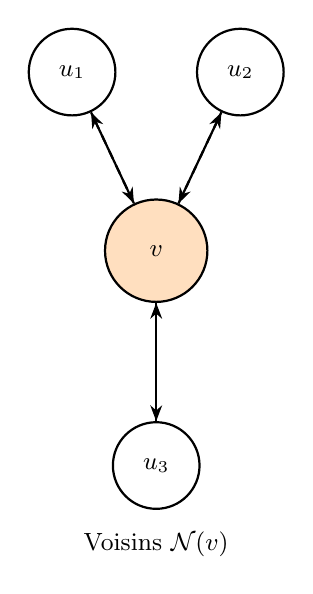
\begin{tikzpicture}[
    font=\small,
    >=Stealth,
    node/.style={circle, draw, thick, minimum size=1.1cm, align=center},
    center/.style={circle, draw, thick, fill=orange!25, minimum size=1.3cm, align=center}
]
\node[center] (c) {$v$};
\node[node, above left=1.4cm and 0.2cm of c] (u1) {$u_1$};
\node[node, above right=1.4cm and 0.2cm of c] (u2) {$u_2$};
\node[node, below=1.5cm of c] (u3) {$u_3$};
\foreach \x in {u1,u2,u3} {
    \draw[thick, -{Stealth[length=2mm]}] (\x) -- (c);
    \draw[thick, dashed, -{Stealth[length=2mm]}] (c) -- (\x);
}
\node[below=0.15cm of u3, align=center] {Voisins $\mathcal{N}(v)$};
\end{tikzpicture}
\end{document}
